

\tikzset{every picture/.style={line width=0.75pt}} %set default line width to 0.75pt        

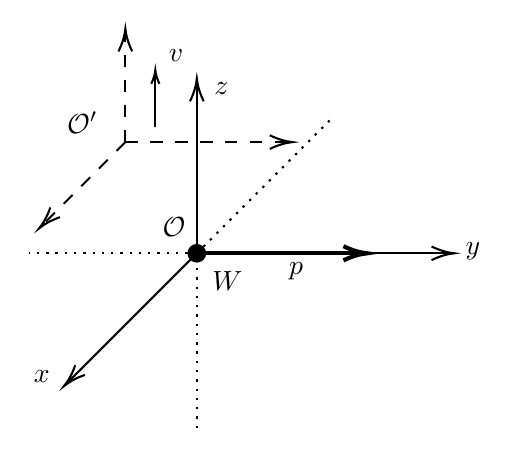
\begin{tikzpicture}[x=0.75pt,y=0.75pt,yscale=-1,xscale=1]
	%uncomment if require: \path (0,197); %set diagram left start at 0, and has height of 197
	
	%Straight Lines [id:da3320609672207786] 
	\draw  [dash pattern={on 0.84pt off 2.51pt}]  (301,109.47) -- (220,109.47) ;
	%Straight Lines [id:da0019449533056650203] 
	\draw    (301,109.47) -- (423.01,109.47) ;
	\draw [shift={(425.01,109.47)}, rotate = 180] [color={rgb, 255:red, 0; green, 0; blue, 0 }  ][line width=0.75]    (10.93,-3.29) .. controls (6.95,-1.4) and (3.31,-0.3) .. (0,0) .. controls (3.31,0.3) and (6.95,1.4) .. (10.93,3.29)   ;
	%Straight Lines [id:da35965824565982163] 
	\draw    (301,109.47) -- (301,27.31) ;
	\draw [shift={(301,25.31)}, rotate = 450] [color={rgb, 255:red, 0; green, 0; blue, 0 }  ][line width=0.75]    (10.93,-3.29) .. controls (6.95,-1.4) and (3.31,-0.3) .. (0,0) .. controls (3.31,0.3) and (6.95,1.4) .. (10.93,3.29)   ;
	%Straight Lines [id:da24691145277823567] 
	\draw    (301,109.47) -- (238.42,172.05) ;
	\draw [shift={(237.01,173.46)}, rotate = 315] [color={rgb, 255:red, 0; green, 0; blue, 0 }  ][line width=0.75]    (10.93,-3.29) .. controls (6.95,-1.4) and (3.31,-0.3) .. (0,0) .. controls (3.31,0.3) and (6.95,1.4) .. (10.93,3.29)   ;
	%Straight Lines [id:da7876238424914852] 
	\draw [line width=1.5]    (301,109.47) -- (380,109.47) ;
	\draw [shift={(383,109.47)}, rotate = 180] [color={rgb, 255:red, 0; green, 0; blue, 0 }  ][line width=1.5]    (11.37,-3.42) .. controls (7.23,-1.45) and (3.44,-0.31) .. (0,0) .. controls (3.44,0.31) and (7.23,1.45) .. (11.37,3.42)   ;
	\draw [shift={(301,109.47)}, rotate = 0] [color={rgb, 255:red, 0; green, 0; blue, 0 }  ][fill={rgb, 255:red, 0; green, 0; blue, 0 }  ][line width=1.5]      (0, 0) circle [x radius= 3.48, y radius= 3.48]   ;
	%Straight Lines [id:da5550885761878284] 
	\draw  [dash pattern={on 0.84pt off 2.51pt}]  (364.99,45.48) -- (301,109.47) ;
	%Straight Lines [id:da6613513151925012] 
	\draw  [dash pattern={on 0.84pt off 2.51pt}]  (301,193.63) -- (301,109.47) ;
	%Straight Lines [id:da21238637764144053] 
	\draw  [dash pattern={on 4.5pt off 4.5pt}]  (266.56,55.91) -- (345.07,55.91) ;
	\draw [shift={(347.07,55.91)}, rotate = 180] [color={rgb, 255:red, 0; green, 0; blue, 0 }  ][line width=0.75]    (10.93,-3.29) .. controls (6.95,-1.4) and (3.31,-0.3) .. (0,0) .. controls (3.31,0.3) and (6.95,1.4) .. (10.93,3.29)   ;
	%Straight Lines [id:da1528335475321898] 
	\draw  [dash pattern={on 4.5pt off 4.5pt}]  (266.56,55.91) -- (266.56,3.27) ;
	\draw [shift={(266.56,1.27)}, rotate = 450] [color={rgb, 255:red, 0; green, 0; blue, 0 }  ][line width=0.75]    (10.93,-3.29) .. controls (6.95,-1.4) and (3.31,-0.3) .. (0,0) .. controls (3.31,0.3) and (6.95,1.4) .. (10.93,3.29)   ;
	%Straight Lines [id:da1861354405272635] 
	\draw  [dash pattern={on 4.5pt off 4.5pt}]  (266.56,55.91) -- (226.42,96.05) ;
	\draw [shift={(225.01,97.46)}, rotate = 315] [color={rgb, 255:red, 0; green, 0; blue, 0 }  ][line width=0.75]    (10.93,-3.29) .. controls (6.95,-1.4) and (3.31,-0.3) .. (0,0) .. controls (3.31,0.3) and (6.95,1.4) .. (10.93,3.29)   ;
	%Straight Lines [id:da4199529155239894] 
	\draw [line width=0.75]    (281,48.47) -- (281,23.27) ;
	\draw [shift={(281,21.27)}, rotate = 450] [color={rgb, 255:red, 0; green, 0; blue, 0 }  ][line width=0.75]    (6.56,-1.97) .. controls (4.17,-0.84) and (1.99,-0.18) .. (0,0) .. controls (1.99,0.18) and (4.17,0.84) .. (6.56,1.97)   ;
	
	% Text Node
	\draw (221,164.58) node [anchor=north west][inner sep=0.75pt]    {$x$};
	% Text Node
	\draw (429,102.58) node [anchor=north west][inner sep=0.75pt]    {$y$};
	% Text Node
	\draw (308,25.58) node [anchor=north west][inner sep=0.75pt]    {$z$};
	% Text Node
	\draw (344,112.47) node [anchor=north west][inner sep=0.75pt]    {$\boldsymbol{p}$};
	% Text Node
	\draw (283,91) node [anchor=north west][inner sep=0.75pt]    {$\mathcal{O}$};
	% Text Node
	\draw (237,40) node [anchor=north west][inner sep=0.75pt]    {$\mathcal{O} '$};
	% Text Node
	\draw (286,10) node [anchor=north west][inner sep=0.75pt]    {$\boldsymbol{v}$};
	% Text Node
	\draw (307,117) node [anchor=north west][inner sep=0.75pt]    {$W$};
	
	
\end{tikzpicture}